\documentclass[conference]{IEEEtran}

% -----------------------------------------------------------------------------
% Packages and Setup
% -----------------------------------------------------------------------------
\usepackage{cite}
\usepackage{amsmath,amssymb,amsfonts}
\usepackage{algorithmic}
\usepackage{graphicx}
\usepackage{textcomp}
\usepackage{xcolor}
\usepackage{booktabs}
\usepackage{array}
\usepackage{tabularx}
\usepackage{url}
\usepackage{microtype}
\usepackage{tikz}
\usetikzlibrary{shapes.geometric, arrows.meta, positioning, calc, patterns, backgrounds}

% Graphics path setup pointing to results directory
\graphicspath{{../../results/}{../results/}{results/}}

% Correct bad hyphenation here
\hyphenation{op-ti-cal net-works semi-con-duc-tor set-as-so-cia-tive direct-mapped}

% -----------------------------------------------------------------------------
% Document Header
% -----------------------------------------------------------------------------
\begin{document}

\title{Design and Performance Analysis of a Two-Way Set-Associative Cache with LRU Replacement Compared with a Direct-Mapped Cache}

\author{
  \IEEEauthorblockN{
    Satyam Kumar,
    Krishna Verma,
    Akshit Vats,
    Chinmay Soni,
    and Lakshya Bapna
  }
  \IEEEauthorblockA{
    Department of Computer Science and Artificial Intelligence\\
    Newton School of Technology
  }
}

\maketitle

% -----------------------------------------------------------------------------
% Abstract and Index Terms
% -----------------------------------------------------------------------------
\begin{abstract}
As semiconductor scaling continues to outpace off-chip dynamic random-access memory (DRAM) access latencies---a fundamental architectural bottleneck formalized as the ``memory wall''---the structural efficiency of processor cache hierarchies plays a decisive role in determining overall system execution throughput. In this paper, we present the cycle-accurate design, microarchitectural modeling, and empirical comparative evaluation of a 128-byte, 2-way set-associative cache with 1-bit Least Recently Used (LRU) replacement against an identically sized direct-mapped cache baseline. Implemented in IEEE 1800-2012 SystemVerilog, both cache microarchitectures utilize a 32-bit byte-addressed memory interface, a 16-byte (4-word) cache-line granularity, single-request blocking execution, and synchronous valid/ready handshake protocols. The memory subsystem is driven by a synchronous multi-cycle latency memory model enforcing refills that execute four consecutive word-read transactions. We subject both architectures to four synthetic access traces in an automated simulation testbench using Icarus Verilog: sequential spatial locality, conflict-heavy ping-pong thrashing, explicit three-address LRU eviction validation, and a realistic mixed-workload trace. Cycle-accurate RTL simulation demonstrates that under severe two-address conflict thrashing, the 2-way set-associative cache achieves a 75.00\% hit rate and 6.25 cycles per access, whereas the direct-mapped cache suffers a 0.00\% hit rate and 17.50 cycles per access. This delivers a 75.00\% reduction in simulated main-memory word reads (8 versus 32 words) and a 64.29\% reduction in measured execution latency (50 versus 140 cycles), corresponding to a $2.80\times$ speedup ratio. These empirical findings demonstrate the effectiveness of set associativity in eliminating conflict misses between concurrently active lines while confirming the deterministic cycle-by-cycle correctness of our hardware LRU eviction controller.
\end{abstract}

\begin{IEEEkeywords}
Cache memory, set-associative cache, direct-mapped cache, least recently used (LRU) replacement, conflict misses, cache thrashing, memory hierarchy, SystemVerilog RTL, cycle-accurate simulation.
\end{IEEEkeywords}

% -----------------------------------------------------------------------------
% Section I: Introduction
% -----------------------------------------------------------------------------
\section{Introduction}
\label{sec:introduction}
\IEEEPARstart{O}{ver} the past four decades, processor core clock frequencies and execution capabilities have escalated at a significantly higher rate than off-chip memory access latencies. This persistent divergence, widely termed the ``memory wall'' by Wulf and McKee~\cite{wulf1995hitting} and rigorously analyzed by Hennessy and Patterson~\cite{hennessy2017computer}, renders high-speed on-chip cache hierarchies indispensable in modern computer architecture. Caches operate as high-speed SRAM buffers interposed between the processor pipeline and high-capacity main storage, relying on the dual principles of \textit{temporal locality} (data referenced recently is likely to be referenced again soon) and \textit{spatial locality} (data physically adjacent to recently referenced addresses is likely to be accessed shortly)~\cite{smith1982cache}.

According to the classical 3C model established by Hill and Smith~\cite{hill1989evaluating}, cache misses are partitioned into three distinct classes:
\begin{enumerate}
    \item \textit{Compulsory (Cold) Misses}: Unavoidable misses occurring on the very first reference to a memory block that has never previously resided in the cache.
    \item \textit{Capacity Misses}: Misses occurring when the active working set of a program exceeds the aggregate physical storage capacity of the cache.
    \item \textit{Conflict (Collision) Misses}: Misses occurring when multiple distinct memory blocks map to the identical cache set or line, forcing premature evictions despite unoccupied capacity elsewhere in the cache.
\end{enumerate}

Direct-mapped caches represent the simplest placement policy: every physical memory address maps to exactly one predetermined cache line. While direct-mapped caches offer minimal hardware area, simple single-comparator tag matching, and rapid hit detection, they are exceptionally susceptible to catastrophic conflict misses. If an instruction loop or data-access pattern alternately references two distinct memory blocks that hash to the same line index, the direct-mapped cache undergoes continuous ping-pong eviction or ``cache thrashing''~\cite{jouppi1990improving, patterson2020riscv}. Under such thrashing conditions, the effective hit rate plunges to zero, degrading system execution throughput to raw memory bus speeds.

Set-associative caches mitigate this vulnerability by organizing cache lines into sets containing $K$ independent slots or ``ways''~\cite{smith1982cache}. In a $K$-way set-associative cache, any given memory block can reside in any of the $K$ ways within its designated set. For $K=2$ (two-way set-associative), up to two conflicting memory blocks can reside simultaneously in on-chip storage without forcing mutual eviction. However, associativity requires a replacement policy to determine which way must be vacated when all ways in a set are valid and a new line must be loaded. The Least Recently Used (LRU) replacement policy represents an effective online heuristic under strong temporal locality, evicting the line that has experienced the longest period of inactivity~\cite{smith1983instruction}. However, as demonstrated in classical literature, LRU performance is workload-dependent and can degrade under cyclic or scanning reference patterns whose active working sets exceed cache associativity. While two-way associativity successfully eliminates conflict misses between two concurrently referenced blocks in the same set, it does not eliminate all conflict misses when three or more active lines compete for the same set, nor does it eliminate capacity misses when the aggregate working set exceeds cache capacity.

In this project, we design, implement, integrate, and empirically validate a cycle-accurate hardware model of both an 8-line (128-byte) baseline direct-mapped cache and a 4-set, 2-way set-associative cache (128-byte total capacity) equipped with a 1-bit LRU replacement controller. Both architectures are developed in IEEE 1800-2012 SystemVerilog and subjected to comprehensive comparative testing against an identical synchronous main memory model under synthetic access patterns using the open-source Icarus Verilog simulation suite. The complete codebase, testbenches, and reproducibility scripts are available in our public GitHub repository: \url{https://github.com/chinmay7980/2-Way-Set-Associative-Cache-with-LRU.git}.

The remainder of this report is organized as follows. Section~\ref{sec:related_work} reviews related literature on cache placement and replacement policies. Section~\ref{sec:architecture} details the proposed hardware architecture, address decoding schemes, datapath organization, and LRU replacement logic. Section~\ref{sec:implementation} outlines the microarchitectural implementation details and finite state machine controllers. Section~\ref{sec:experiments} presents empirical simulation results, quantitative metrics, and architectural discussion. Section~\ref{sec:contributions} documents the individual engineering contributions across all five team members. Section~\ref{sec:conclusion} concludes the paper and outlines future extensions.

% -----------------------------------------------------------------------------
% Section II: Related Work / Literature Review
% -----------------------------------------------------------------------------
\section{Related Work and Literature Review}
\label{sec:related_work}

The architecture and optimization of cache memories have been extensively studied since the foundational surveys by Alan Jay Smith~\cite{smith1982cache}. Smith established the fundamental taxonomy of cache placement rules, write strategies (write-through versus write-back), fetch algorithms (demand fetch versus prefetching), and block replacement schemes, demonstrating that miss ratios decrease monotonically with increased associativity, albeit with diminishing returns.

In their seminal treatise on cache associativity, Hill and Smith~\cite{hill1989evaluating} quantitatively evaluated the performance trade-offs of varying degrees of associativity across real-world instruction and data workloads. They formulated the well-known ``$2:1$ cache rule of thumb,'' which posits that a direct-mapped cache of size $N$ exhibits an empirical miss rate approximately equal to a 2-way set-associative cache of size $N/2$. However, Hill and Smith emphasized that set associativity incurs hardware overhead: parallel tag comparators, wider data multiplexers, replacement state logic, and increased critical path delay during the tag-matching phase. Consequently, direct-mapped caches were historically favored in early pipelined RISC architectures where single-cycle access latency was the dominant design objective.

Jouppi~\cite{jouppi1990improving} analyzed the specific nature of conflict misses in direct-mapped architectures, demonstrating that high-performance RISC processors frequently experience severe conflict thrashing due to spatial and temporal interference between instruction streams and data structures. Jouppi proposed augmenting direct-mapped caches with a small, fully associative ``victim cache'' to rescue recently evicted blocks, demonstrating that even a minimal 4-entry associative buffer dramatically reduces conflict penalties. This work highlighted that providing alternative placement options for conflicting addresses yields substantial performance dividends.

Replacement policy selection is equally critical. In their comparative evaluation of cache replacement policies, Smith and Goodman~\cite{smith1983instruction} contrasted LRU, First-In First-Out (FIFO), and Random replacement across diverse working sets. Their empirical results demonstrated that true LRU often achieves lower miss rates than FIFO or Random for workloads exhibiting pronounced temporal locality by exploiting the recency of active program references. Nonetheless, they observed that LRU is not universally optimal across all memory reference patterns, particularly under streaming sequences or cyclical loops where lines are repeatedly evicted immediately prior to reuse. For a 2-way set-associative cache, full LRU requires only a single tracking bit per set, eliminating the multi-bit matrix overhead associated with higher-order associativities ($K \ge 4$).

Modern computer architecture textbooks, such as Hennessy and Patterson~\cite{hennessy2017computer} and Patterson and Hennessy~\cite{patterson2020riscv}, synthesize these principles into standardized design methodologies. They demonstrate that for contemporary resource-constrained embedded systems, edge Internet-of-Things (IoT) processors, and microcontroller execution units, a 2-way set-associative organization represents a well-balanced trade-off between structural silicon overhead and conflict miss mitigation. Our investigation builds directly upon these theoretical insights, validating their concrete RTL realization and performance characteristics through cycle-accurate SystemVerilog simulation.

% -----------------------------------------------------------------------------
% Section III: Proposed Hardware Architecture
% -----------------------------------------------------------------------------
\section{Proposed Solution and Hardware Architecture}
\label{sec:architecture}

\subsection{Overall Subsystem Organization}
The subsystem developed in this project consists of two distinct cache microarchitectures: a baseline Direct-Mapped Cache (\texttt{direct\_mapped\_cache}) and a modular Two-Way Set-Associative Cache (\texttt{cache\_2way\_top}), both interfacing with a synchronous main memory module (\texttt{simple\_main\_memory}) and an automated verification testbench. Fig.~\ref{fig:sys_arch} illustrates the top-level subsystem block diagram.

\begin{figure*}[t!]
\centering
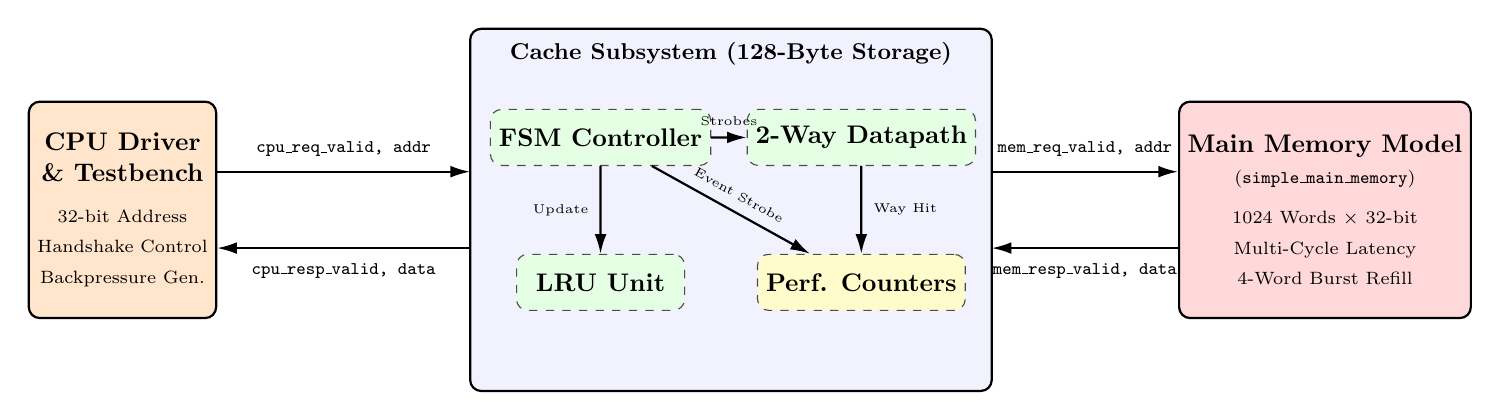
\begin{tikzpicture}[
    scale=0.92, every node/.style={scale=0.92},
    box/.style={rectangle, draw=black, thick, fill=blue!10, align=center, rounded corners, minimum height=3.0em, minimum width=7.0em},
    subbox/.style={rectangle, draw=black!70, dashed, fill=green!10, align=center, rounded corners, minimum height=2.2em, minimum width=6.6em},
    line/.style={draw, -{Latex[length=2.5mm,width=1.5mm]}, thick}
]

% CPU / TB Block
\node[box, fill=orange!20, minimum height=8.5em, minimum width=7.2em] (cpu) at (-1.4, 0) {
    \textbf{CPU Driver}\\
    \textbf{\& Testbench}\\[0.4em]
    \scriptsize 32-bit Address\\
    \scriptsize Handshake Control\\
    \scriptsize Backpressure Gen.
};

% Cache Subsystem Container
\draw[thick, fill=blue!5, rounded corners] (3.4, -2.5) rectangle (10.6, 2.5);
\node[font=\bfseries\small] at (7.0, 2.15) {Cache Subsystem (128-Byte Storage)};

% Submodules inside 2-Way Top arranged in clean 2x2 grid
\node[subbox] (ctrl) at (5.2, 1.0) {\textbf{FSM Controller}};
\node[subbox] (dp)   at (8.8, 1.0) {\textbf{2-Way Datapath}};
\node[subbox] (lru)  at (5.2, -1.0) {\textbf{LRU Unit}};
\node[subbox, fill=yellow!20] (cnt)  at (8.8, -1.0) {\textbf{Perf. Counters}};

% Memory Block
\node[box, fill=red!15, minimum height=8.5em, minimum width=8.5em] (mem) at (15.2, 0) {
    \textbf{Main Memory Model}\\
    \scriptsize (\texttt{simple\_main\_memory})\\[0.4em]
    \scriptsize 1024 Words $\times$ 32-bit\\
    \scriptsize Multi-Cycle Latency\\
    \scriptsize 4-Word Burst Refill
};

% CPU to Cache buses with increased label clearance
\draw[line] ([yshift=1.5em]cpu.east) -- node[above=2pt, font=\scriptsize, align=center] {\texttt{cpu\_req\_valid, addr}} ([yshift=1.5em]3.4, 0);
\draw[line] ([yshift=-1.5em]3.4, 0) -- node[below=2pt, font=\scriptsize, align=center] {\texttt{cpu\_resp\_valid, data}} ([yshift=-1.5em]cpu.east);

% Internal Connections without line crossings
\draw[line] (ctrl) -- node[above=1pt, font=\tiny] {Strobes} (dp);
\draw[line] (ctrl) -- node[left=1pt, font=\tiny] {Update} (lru);
\draw[line] (dp) -- node[right=1pt, font=\tiny] {Way Hit} (cnt);
\draw[line] (ctrl) -- node[above=1pt, font=\tiny, sloped] {Event Strobe} (cnt);

% Cache to Memory buses with increased label clearance
\draw[line] ([yshift=1.5em]10.6, 0) -- node[above=2pt, font=\scriptsize, align=center] {\texttt{mem\_req\_valid, addr}} ([yshift=1.5em]mem.west);
\draw[line] ([yshift=-1.5em]mem.west) -- node[below=2pt, font=\scriptsize, align=center] {\texttt{mem\_resp\_valid, data}} ([yshift=-1.5em]10.6, 0);

\end{tikzpicture}
\caption{Subsystem block diagram depicting the CPU driver, the modular 2-way set-associative cache with decoupled datapath, controller, LRU unit, and performance counters, and the synchronous main memory simulation model.}
\label{fig:sys_arch}
\end{figure*}

Both caches share a standardized, synchronous active-low reset interface (\texttt{rst\_n}) and run on a common system clock (\texttt{clk}). The CPU interface implements a single-request blocking protocol:
\begin{itemize}
    \item Input request: \texttt{cpu\_req\_valid} (1 bit), \texttt{cpu\_req\_addr} (32 bits).
    \item Request acceptance: \texttt{cpu\_req\_ready} (1 bit).
    \item Output response: \texttt{cpu\_resp\_valid} (1 bit), \texttt{cpu\_resp\_data} (32 bits).
    \item Response acceptance: \texttt{cpu\_resp\_ready} (1 bit).
\end{itemize}
Handshakes conform to standard ready/valid conventions: a transfer commits on the active clock edge if and only if both \texttt{valid} and \texttt{ready} are asserted simultaneously. The cache guarantees that once \texttt{cpu\_resp\_valid} is asserted, both the valid signal and the corresponding \texttt{cpu\_resp\_data} remain stable until the CPU asserts \texttt{cpu\_resp\_ready}.

\subsection{Architectural Parameters and Address Mapping}
To ensure a strictly fair comparative evaluation, both cache microarchitectures are configured with an identical total storage capacity of 128 bytes, partitioned into 16-byte cache lines. Each cache line comprises four 32-bit words. Table~\ref{tab:hardware_params} summarizes the complete hardware parameterization defined in \texttt{rtl/cache\_pkg.sv}.

\begin{table}[htbp]
\caption{Microarchitectural Configuration and Parameter Comparison}
\label{tab:hardware_params}
\centering
\resizebox{\columnwidth}{!}{%
\begin{tabular}{lcc}
\toprule
\textbf{Architectural Parameter} & \textbf{Direct-Mapped} & \textbf{2-Way Set-Assoc.} \\
\midrule
Total Data Capacity & 128 Bytes & 128 Bytes \\
Cache Line Granularity & 16 Bytes & 16 Bytes \\
Words per Cache Line & 4 Words (32-bit) & 4 Words (32-bit) \\
Number of Lines / Sets & 8 Lines & 4 Sets \\
Associativity Degree ($K$) & 1 (Direct-Mapped) & 2 Ways per Set \\
Total Cache Lines & 8 Lines & 8 Lines \\
Byte Offset Field & Bits $[1:0]$ (2 bits) & Bits $[1:0]$ (2 bits) \\
Word Offset Field & Bits $[3:2]$ (2 bits) & Bits $[3:2]$ (2 bits) \\
Set / Line Index Field & Bits $[6:4]$ (3 bits) & Bits $[5:4]$ (2 bits) \\
Tag Address Field & Bits $[31:7]$ (25 bits) & Bits $[31:6]$ (26 bits) \\
Tag Storage Overhead & $8 \times 25 = 200$ bits & $8 \times 26 = 208$ bits \\
Valid Bits & 8 bits (1 per line) & 8 bits (1 per way) \\
Replacement State & None & 4 bits (1 per set) \\
Replacement Policy & Overwrite / Evict & True LRU (1 bit/set) \\
Access Mode & Read-Only / Blocking & Read-Only / Blocking \\
Refill Protocol & 4-Word Synchronous & 4-Word Synchronous \\
\bottomrule
\end{tabular}%
}
\end{table}

Fig.~\ref{fig:addr_mapping} illustrates the physical 32-bit byte-address partitioning for both microarchitectures. Because the 2-way set-associative cache groups its eight lines into four sets of two ways each, it requires a 2-bit set index (\texttt{address[5:4]}), expanding its tag field to 26 bits (\texttt{address[31:6]}). In contrast, the direct-mapped cache indexes across all eight independent lines, requiring a 3-bit index (\texttt{address[6:4]}) and a 25-bit tag (\texttt{address[31:7]}). Both designs use \texttt{address[3:2]} to select one of the four 32-bit words within a line, while byte-offset bits \texttt{address[1:0]} are ignored during aligned word transfers.

\begin{figure}[htbp]
\centering
\resizebox{\columnwidth}{!}{%
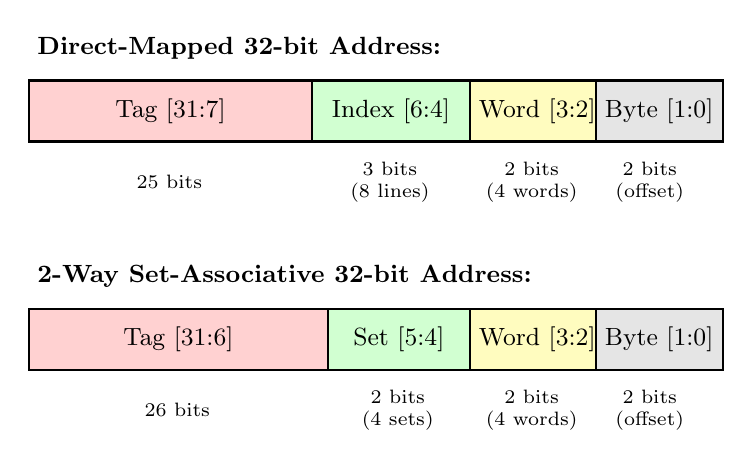
\begin{tikzpicture}[
    box/.style={draw=black, thick, minimum height=2.2em, align=center, font=\small},
    lbl/.style={font=\scriptsize, align=center, text=black}
]

% ---------------- Direct-Mapped Address ----------------
\node[anchor=west, font=\bfseries\small] at (0, 2.5) {Direct-Mapped 32-bit Address:};

% Fields (Total width = 8.6cm)
\node[box, fill=red!18, minimum width=3.6cm, anchor=west] (dm_tag) at (0, 1.7) {Tag [31:7]};
\node[box, fill=green!18, minimum width=2.0cm, anchor=west] (dm_idx) at (3.6, 1.7) {Index [6:4]};
\node[box, fill=yellow!25, minimum width=1.6cm, anchor=west] (dm_word) at (5.6, 1.7) {Word [3:2]};
\node[box, fill=gray!20, minimum width=1.4cm, anchor=west] (dm_byte) at (7.2, 1.7) {Byte [1:0]};

% Sub-labels (centered below each field)
\node[lbl] at (1.8, 0.8) {25 bits};
\node[lbl] at (4.6, 0.8) {3 bits\\(8 lines)};
\node[lbl] at (6.4, 0.8) {2 bits\\(4 words)};
\node[lbl] at (7.9, 0.8) {2 bits\\(offset)};

% ---------------- 2-Way Set-Associative Address ----------------
\node[anchor=west, font=\bfseries\small] at (0, -0.4) {2-Way Set-Associative 32-bit Address:};

% Fields (Total width = 8.6cm)
\node[box, fill=red!18, minimum width=3.8cm, anchor=west] (sa_tag) at (0, -1.2) {Tag [31:6]};
\node[box, fill=green!18, minimum width=1.8cm, anchor=west] (sa_idx) at (3.8, -1.2) {Set [5:4]};
\node[box, fill=yellow!25, minimum width=1.6cm, anchor=west] (sa_word) at (5.6, -1.2) {Word [3:2]};
\node[box, fill=gray!20, minimum width=1.4cm, anchor=west] (sa_byte) at (7.2, -1.2) {Byte [1:0]};

% Sub-labels (centered below each field)
\node[lbl] at (1.9, -2.1) {26 bits};
\node[lbl] at (4.7, -2.1) {2 bits\\(4 sets)};
\node[lbl] at (6.4, -2.1) {2 bits\\(4 words)};
\node[lbl] at (7.9, -2.1) {2 bits\\(offset)};

\end{tikzpicture}%
}
\caption{Comparative 32-bit address field partitioning between direct-mapped (25-bit tag, 3-bit line index) and 2-way set-associative (26-bit tag, 2-bit set index) configurations.}
\label{fig:addr_mapping}
\end{figure}

\subsection{Two-Way Set-Associative Datapath Organization}
The two-way set-associative datapath is implemented in \texttt{rtl/cache\_2way\_datapath.sv}. It decouples storage arrays and tag-matching comparators from control sequencing. The datapath instantiates two parallel ways (Way~0 and Way~1) across four sets:
\begin{itemize}
    \item Way~0 Storage: \texttt{data\_array\_w0[0:3][0:3]}, \texttt{tag\_array\_w0[0:3]}, and \texttt{valid\_array\_w0[0:3]}.
    \item Way~1 Storage: \texttt{data\_array\_w1[0:3][0:3]}, \texttt{tag\_array\_w1[0:3]}, and \texttt{valid\_array\_w1[0:3]}.
\end{itemize}

Fig.~\ref{fig:datapath_diagram} depicts the parallel tag comparison and data selection circuitry. For a registered set index \texttt{set\_idx = address[5:4]}, the datapath performs concurrent tag comparisons across both ways:
\begin{align}
\text{hit\_w0} &= \text{valid\_w0}[\text{set}] \land (\text{tag\_w0}[\text{set}] == \text{req\_tag}) \\
\text{hit\_w1} &= \text{valid\_w1}[\text{set}] \land (\text{tag\_w1}[\text{set}] == \text{req\_tag}) \\
\text{cache\_hit} &= \text{hit\_w0} \lor \text{hit\_w1}
\end{align}

\begin{figure}[htbp]
\centering
\resizebox{\columnwidth}{!}{%
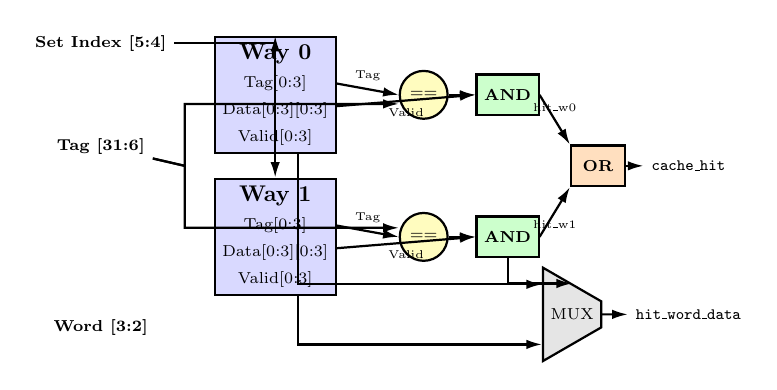
\begin{tikzpicture}[
    scale=0.82, every node/.style={scale=0.82},
    arr/.style={rectangle, draw=black, thick, fill=blue!15, minimum height=3.5em, minimum width=4.8em, align=center},
    comp/.style={circle, draw=black, thick, fill=yellow!25, minimum size=1.8em, align=center, font=\scriptsize\bfseries},
    mux/.style={trapezium, draw=black, thick, fill=gray!20, minimum height=1.6em, align=center, shape border rotate=270, font=\scriptsize},
    gate/.style={rectangle, draw=black, thick, fill=green!20, minimum height=1.8em, minimum width=2.4em, align=center, font=\scriptsize\bfseries},
    line/.style={draw, -{Latex[length=2.0mm,width=1.2mm]}, thick}
]

% Inputs
\node[font=\bfseries\scriptsize] (set_in) at (-0.5, 2.0) {Set Index [5:4]};
\node[font=\bfseries\scriptsize] (tag_in) at (-0.5, 0.4) {Tag [31:6]};
\node[font=\bfseries\scriptsize] (word_in) at (-0.5, -2.4) {Word [3:2]};

% Way 0 Block
\node[arr] (w0) at (2.2, 1.2) {\textbf{Way 0}\\ \scriptsize Tag[0:3]\\ \scriptsize Data[0:3][0:3]\\ \scriptsize Valid[0:3]};

% Way 1 Block
\node[arr] (w1) at (2.2, -1.0) {\textbf{Way 1}\\ \scriptsize Tag[0:3]\\ \scriptsize Data[0:3][0:3]\\ \scriptsize Valid[0:3]};

% Comparators
\node[comp] (cmp0) at (4.5, 1.2) {$==$};
\node[comp] (cmp1) at (4.5, -1.0) {$==$};

% Hit Gates
\node[gate] (and0) at (5.8, 1.2) {AND};
\node[gate] (and1) at (5.8, -1.0) {AND};

% OR Gate
\node[gate, fill=orange!25] (or_hit) at (7.2, 0.1) {OR};
\node[font=\bfseries\scriptsize] (hit_out) at (8.6, 0.1) {\texttt{cache\_hit}};

% Data Mux
\node[mux] (dmux) at (6.8, -2.2) {MUX};
\node[font=\bfseries\scriptsize] (data_out) at (8.6, -2.2) {\texttt{hit\_word\_data}};

% Signal routing
\draw[line] (set_in) -| (w0.north);
\draw[line] (set_in) -| (w1.north);
\draw[line] (tag_in) -- (0.8, 0.1) |- ([yshift=-0.4em]cmp0.west);
\draw[line] (tag_in) -- (0.8, 0.1) |- ([yshift=0.4em]cmp1.west);

\draw[line] ([yshift=0.5em]w0.east) -- node[above, font=\tiny] {Tag} (cmp0.west);
\draw[line] ([yshift=0.5em]w1.east) -- node[above, font=\tiny] {Tag} (cmp1.west);

\draw[line] (cmp0.east) -- (and0.west);
\draw[line] (cmp1.east) -- (and1.west);

\draw[line] ([yshift=-0.5em]w0.east) -- node[below, font=\tiny] {Valid} (and0.west);
\draw[line] ([yshift=-0.5em]w1.east) -- node[below, font=\tiny] {Valid} (and1.west);

\draw[line] (and0.east) -- node[above, font=\tiny] {hit\_w0} (or_hit.north west);
\draw[line] (and1.east) -- node[below, font=\tiny] {hit\_w1} (or_hit.south west);
\draw[line] (or_hit.east) -- (hit_out);

\draw[line] ([xshift=1em]w0.south) |- (dmux.north west);
\draw[line] ([xshift=1em]w1.south) |- (dmux.south west);
\draw[line] (and1.south) |- (dmux.north);
\draw[line] (dmux.east) -- (data_out);

\end{tikzpicture}%
}
\caption{Two-Way Set-Associative datapath microarchitecture illustrating parallel tag matching across Way~0 and Way~1, hit logic generation, and way selection multiplexing.}
\label{fig:datapath_diagram}
\end{figure}

Because a memory address can match at most one valid way at any given instant (guaranteed by our mutual-exclusion allocation invariants), \texttt{hit\_w0} and \texttt{hit\_w1} are strictly mutually exclusive. If \texttt{hit\_w0} is asserted, the way multiplexer routes the word selected from Way~0; if \texttt{hit\_w1} is asserted, it routes the word selected from Way~1.

\subsection{1-Bit LRU Replacement Controller}
The LRU replacement controller is implemented as an independent hardware module in \texttt{rtl/lru\_controller.sv}. For a 2-way set-associative cache, full LRU tracking requires exactly 1 bit of replacement state per set:
\begin{equation}
\text{LRU Array: } \text{lru\_bits}[0:3], \quad \text{Width} = 1\text{ bit per set}
\end{equation}

The architectural convention adopted throughout our design is strictly formalized as:
\begin{itemize}
    \item $\text{lru\_bits}[\text{set}] = 0$: Way~0 was least recently accessed; Way~0 is the replacement candidate.
    \item $\text{lru\_bits}[\text{set}] = 1$: Way~1 was least recently accessed; Way~1 is the replacement candidate.
\end{itemize}

Whenever an access occurs to a set (either a cache hit during \texttt{LOOKUP} or a newly completed refill during \texttt{RESP}), the replacement bit is deterministically updated:
\begin{equation}
\text{lru\_bits}[\text{set}] \leftarrow \begin{cases}
1, & \text{if Way 0 accessed}, \\
0, & \text{if Way 1 accessed}.
\end{cases}
\end{equation}

Crucially, the replacement controller enforces an \textit{invalid-first allocation priority} before consulting the LRU bit:
\begin{equation}
\text{replace\_way} = \begin{cases}
0, & \text{if } \neg\text{valid0}, \\
1, & \text{if } \text{valid0} \land \neg\text{valid1}, \\
\text{lru\_victim}, & \text{if } \text{valid0} \land \text{valid1}.
\end{cases}
\end{equation}
This hardware rule guarantees that empty (invalid) cache ways are always populated first upon initial cold accesses, entirely preventing premature evictions of valid working data.

% -----------------------------------------------------------------------------
% Section IV: Implementation Details
% -----------------------------------------------------------------------------
\section{Implementation Details}
\label{sec:implementation}

\subsection{Finite State Machine (FSM) Design}
The sequencing of cache operations is governed by a synchronous Mealy/Moore finite state machine implemented in \texttt{rtl/cache\_2way\_controller.sv}. The FSM comprises five orthogonal states, depicted in Fig.~\ref{fig:fsm_diagram}:

\begin{figure}[htbp]
\centering
\resizebox{0.96\columnwidth}{!}{%
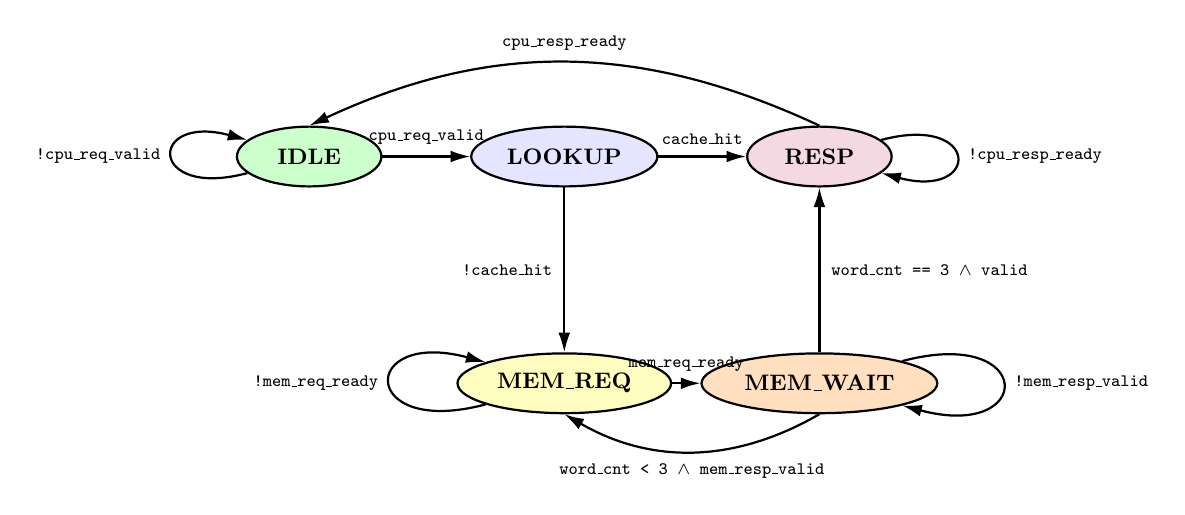
\begin{tikzpicture}[
    scale=0.9, every node/.style={scale=0.9},
    state/.style={ellipse, draw=black, thick, fill=blue!10, align=center, minimum height=2.4em, minimum width=5.8em, font=\bfseries\small},
    line/.style={draw, -{Latex[length=2.5mm,width=1.5mm]}, thick},
    lbl/.style={font=\scriptsize, align=center, fill=white, inner sep=2pt}
]

% States layout in 2 horizontal rows
\node[state, fill=green!20] (idle)   at (0, 3.2) {IDLE};
\node[state]                (lookup) at (3.6, 3.2) {LOOKUP};
\node[state, fill=purple!15](resp)   at (7.2, 3.2) {RESP};
\node[state, fill=yellow!25](req)    at (3.6, 0) {MEM\_REQ};
\node[state, fill=orange!25](waitst) at (7.2, 0) {MEM\_WAIT};

% Forward transitions
\draw[line] (idle) -- node[above=1pt, font=\scriptsize] {\texttt{cpu\_req\_valid}} (lookup);
\draw[line] (lookup) -- node[above=1pt, font=\scriptsize] {\texttt{cache\_hit}} (resp);
\draw[line] (lookup) -- node[left=1pt, font=\scriptsize] {\texttt{!cache\_hit}} (req);
\draw[line] (req) -- node[above=1pt, font=\scriptsize] {\texttt{mem\_req\_ready}} (waitst);

% Refill word loop between MEM_WAIT and MEM_REQ
\draw[line] (waitst.south) to [bend left=30] node[below=1pt, font=\scriptsize] {\texttt{word\_cnt < 3 $\land$ mem\_resp\_valid}} (req.south);

% Refill completion transition to RESP
\draw[line] (waitst) -- node[right=1pt, font=\scriptsize] {\texttt{word\_cnt == 3 $\land$ valid}} (resp);

% Return transition from RESP to IDLE
\draw[line] (resp.north) to [bend right=25] node[above=1pt, font=\scriptsize] {\texttt{cpu\_resp\_ready}} (idle.north);

% Self-loops cleanly positioned outside
\draw[line] (idle) to [loop left] node[left=1pt, font=\scriptsize] {\texttt{!cpu\_req\_valid}} (idle);
\draw[line] (req) to [loop left] node[left=1pt, font=\scriptsize] {\texttt{!mem\_req\_ready}} (req);
\draw[line] (waitst) to [loop right] node[right=1pt, font=\scriptsize] {\texttt{!mem\_resp\_valid}} (waitst);
\draw[line] (resp) to [loop right] node[right=1pt, font=\scriptsize] {\texttt{!cpu\_resp\_ready}} (resp);

\end{tikzpicture}%
}
\caption{Finite State Machine (FSM) state transition diagram for the blocking cache controller, depicting lookup, 4-word burst refill loop, and handshake synchronization.}
\label{fig:fsm_diagram}
\end{figure}

\begin{enumerate}
    \item \textbf{IDLE}: The cache asserts \texttt{cpu\_req\_ready = 1}. Upon detecting \texttt{cpu\_req\_valid = 1}, the controller latches \texttt{cpu\_req\_addr} into internal registers and transitions to \texttt{LOOKUP}.
    \item \textbf{LOOKUP}: The datapath performs parallel tag comparison. If \texttt{cache\_hit} is true, \texttt{hit\_count} increments, the LRU state updates to reflect the accessed way, and the FSM branches directly to \texttt{RESP}. If \texttt{cache\_hit} is false, \texttt{miss\_count} increments, the victim way is evaluated via \texttt{replace\_way}, the word refill counter \texttt{refill\_word\_cnt} is reset to 0, and the FSM transitions to \texttt{MEM\_REQ}.
    \item \textbf{MEM\_REQ}: The controller generates a word read request to main memory, asserting \texttt{mem\_req\_valid = 1} with \texttt{mem\_req\_addr} aligned to the 16-byte boundary. When the memory asserts \texttt{mem\_req\_ready = 1}, \texttt{mem\_word\_read\_count} increments, and the FSM transitions to \texttt{MEM\_WAIT}.
    \item \textbf{MEM\_WAIT}: The controller sets \texttt{mem\_resp\_ready = 1} and waits for \texttt{mem\_resp\_valid = 1}. Upon receiving data, the 32-bit word is written to \texttt{data\_array} at \texttt{[replace\_way][latched\_set][refill\_word\_cnt]}. If \texttt{refill\_word\_cnt < 3}, \texttt{refill\_word\_cnt} increments, and the FSM loops back to \texttt{MEM\_REQ} for the next word. When \texttt{refill\_word\_cnt == 3}, the final word is written, the tag array is updated with \texttt{latched\_tag}, the valid bit is set, the LRU bit is updated to point away from \texttt{replace\_way}, and the FSM transitions to \texttt{RESP}.
    \item \textbf{RESP}: The cache drives \texttt{cpu\_resp\_valid = 1} and outputs the requested 32-bit word on \texttt{cpu\_resp\_data}. Both signals remain asserted until the CPU raises \texttt{cpu\_resp\_ready = 1}, whereupon the FSM returns to \texttt{IDLE}.
\end{enumerate}

\subsection{Main Memory Simulation Model and Refill Protocol}
Main memory is modeled in \texttt{sim/simple\_main\_memory.sv} as a behavioral synchronous memory simulation model containing 1024 32-bit words (4~KB addressable space). Memory data initialization follows a deterministic arithmetic pattern:
\begin{equation}
\text{memory\_array}[i] = 32'\text{hA5000000} \oplus i, \quad i \in [0, 1023]
\end{equation}
This deterministic structure allows the verification environment to independently calculate the exact expected data word for any byte address:
\begin{equation}
\text{Expected Data} = 32'\text{hA5000000} \oplus \left( \frac{\text{address}}{4} \right)
\end{equation}
The memory model implements a parameterized access latency (\texttt{LATENCY\_CYCLES = 2}) and request gap (\texttt{REQUEST\_GAP\_CYCLES = 1}), emulating multi-cycle timing penalties in simulation. When a cache line refill occurs, the cache controller executes four consecutive word-read transactions to memory addresses aligned to 16-byte boundaries ($\text{word\_idx} = 0, 1, 2, 3$).

\subsection{RTL Source Inventory}
Table~\ref{tab:rtl_modules} lists the SystemVerilog source modules comprising the implementation.

\begin{table}[htbp]
\caption{SystemVerilog RTL Implementation Modules and Descriptions}
\label{tab:rtl_modules}
\centering
\begin{tabularx}{\columnwidth}{lX}
\toprule
\textbf{Source File} & \textbf{Microarchitectural Role and Features} \\
\midrule
\texttt{rtl/cache\_pkg.sv} & SystemVerilog package containing all global architectural parameters, bit widths, constants, and state declarations. \\
\addlinespace[0.3em]
\texttt{rtl/direct\_mapped\_cache.sv} & Baseline 8-line direct-mapped cache incorporating integrated storage arrays, single tag comparator, blocking FSM, and counters. \\
\addlinespace[0.3em]
\texttt{rtl/cache\_2way\_datapath.sv} & Modular datapath containing dual-way storage arrays, parallel tag comparators, word extractors, and write-enable demuxes. \\
\addlinespace[0.3em]
\texttt{rtl/lru\_controller.sv} & 1-bit LRU replacement engine managing 4 set bits, implementing invalid-first priority and access-driven state updates. \\
\addlinespace[0.3em]
\texttt{rtl/cache\_2way\_controller.sv} & Central 5-state FSM sequencer governing handshakes, memory burst generation, array updates, and counter tracking. \\
\addlinespace[0.3em]
\texttt{rtl/cache\_2way\_top.sv} & Structural top-level wrapper interconnecting datapath, controller, LRU unit, and performance counter registers. \\
\addlinespace[0.3em]
\texttt{sim/simple\_main\_memory.sv} & Synchronous 1024-word memory model with parameterized multi-cycle latency and deterministic data generation. \\
\bottomrule
\end{tabularx}
\end{table}

% -----------------------------------------------------------------------------
% Section V: Results and Discussion
% -----------------------------------------------------------------------------
\section{Results and Discussion}
\label{sec:experiments}

\begin{figure*}[t!]
\centering
\begin{minipage}{0.32\textwidth}
  \centering
  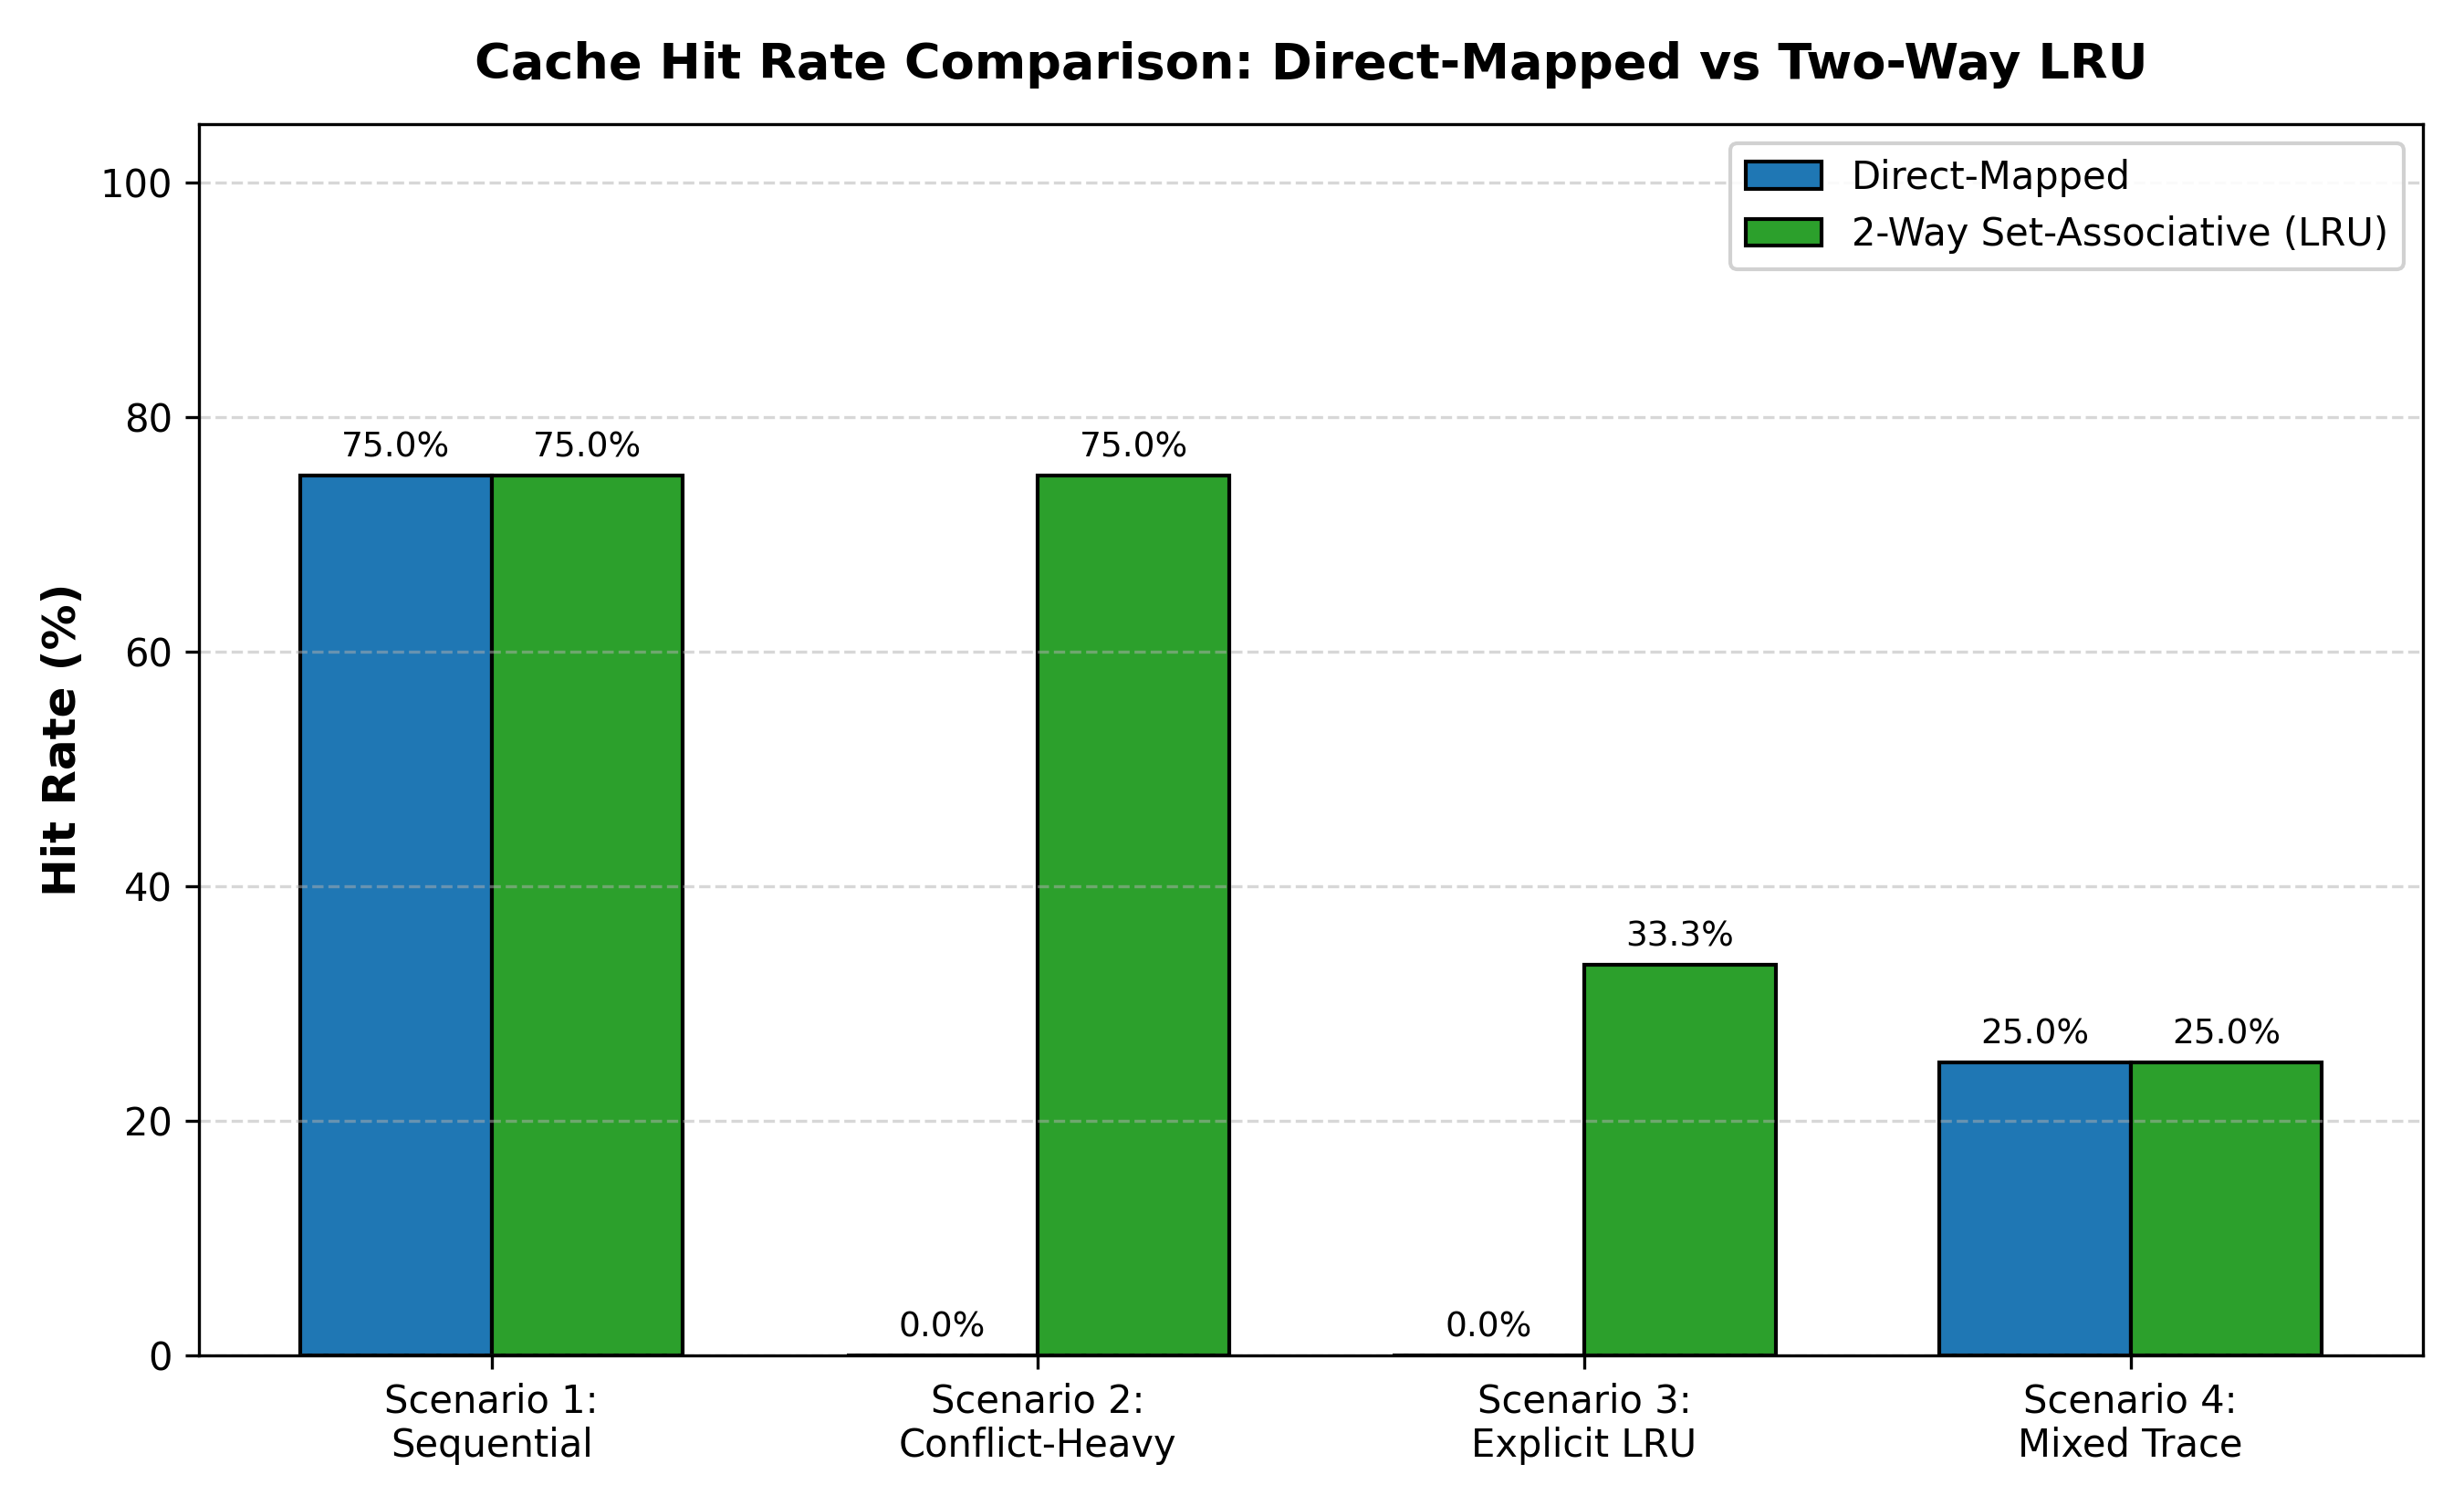
\includegraphics[width=0.92\linewidth]{hit_rate_comparison.png}
  \vspace{0.15em}
  \centerline{\small (a) Cache Hit Rate (\%)}
\end{minipage}\hfill
\begin{minipage}{0.32\textwidth}
  \centering
  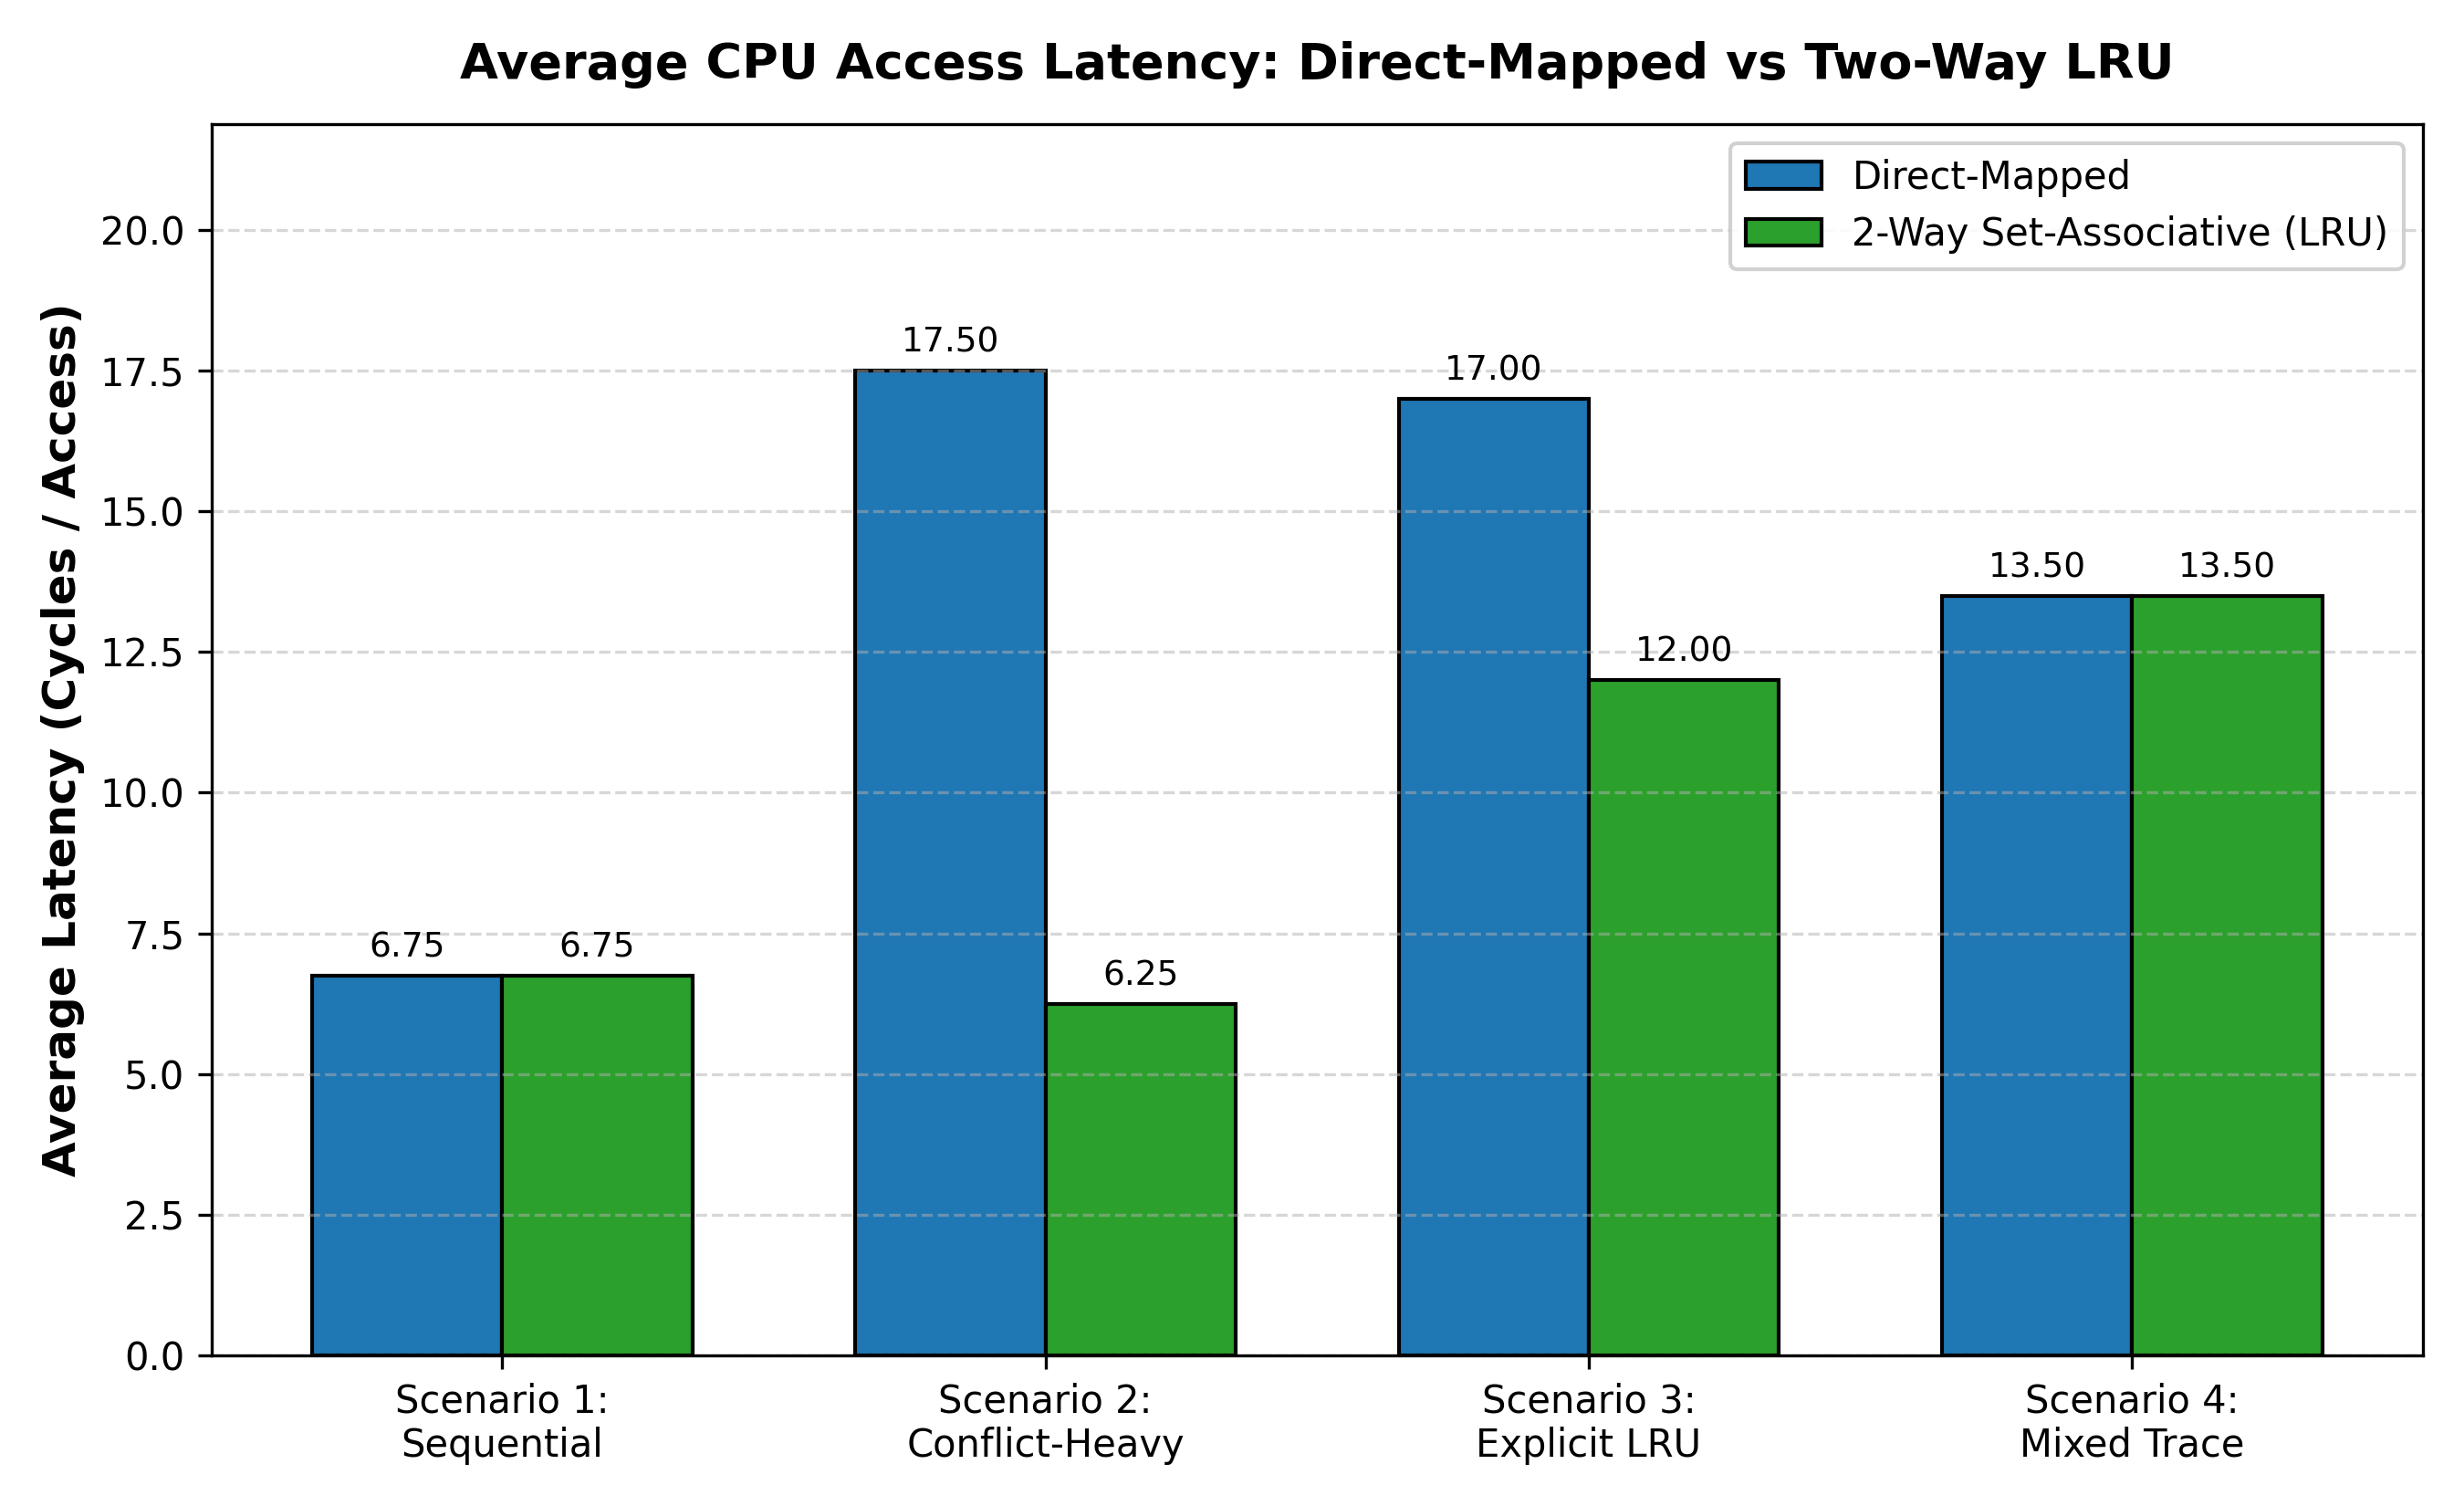
\includegraphics[width=0.92\linewidth]{average_latency_comparison.png}
  \vspace{0.15em}
  \centerline{\small (b) Average Latency (Cycles/Access)}
\end{minipage}\hfill
\begin{minipage}{0.32\textwidth}
  \centering
  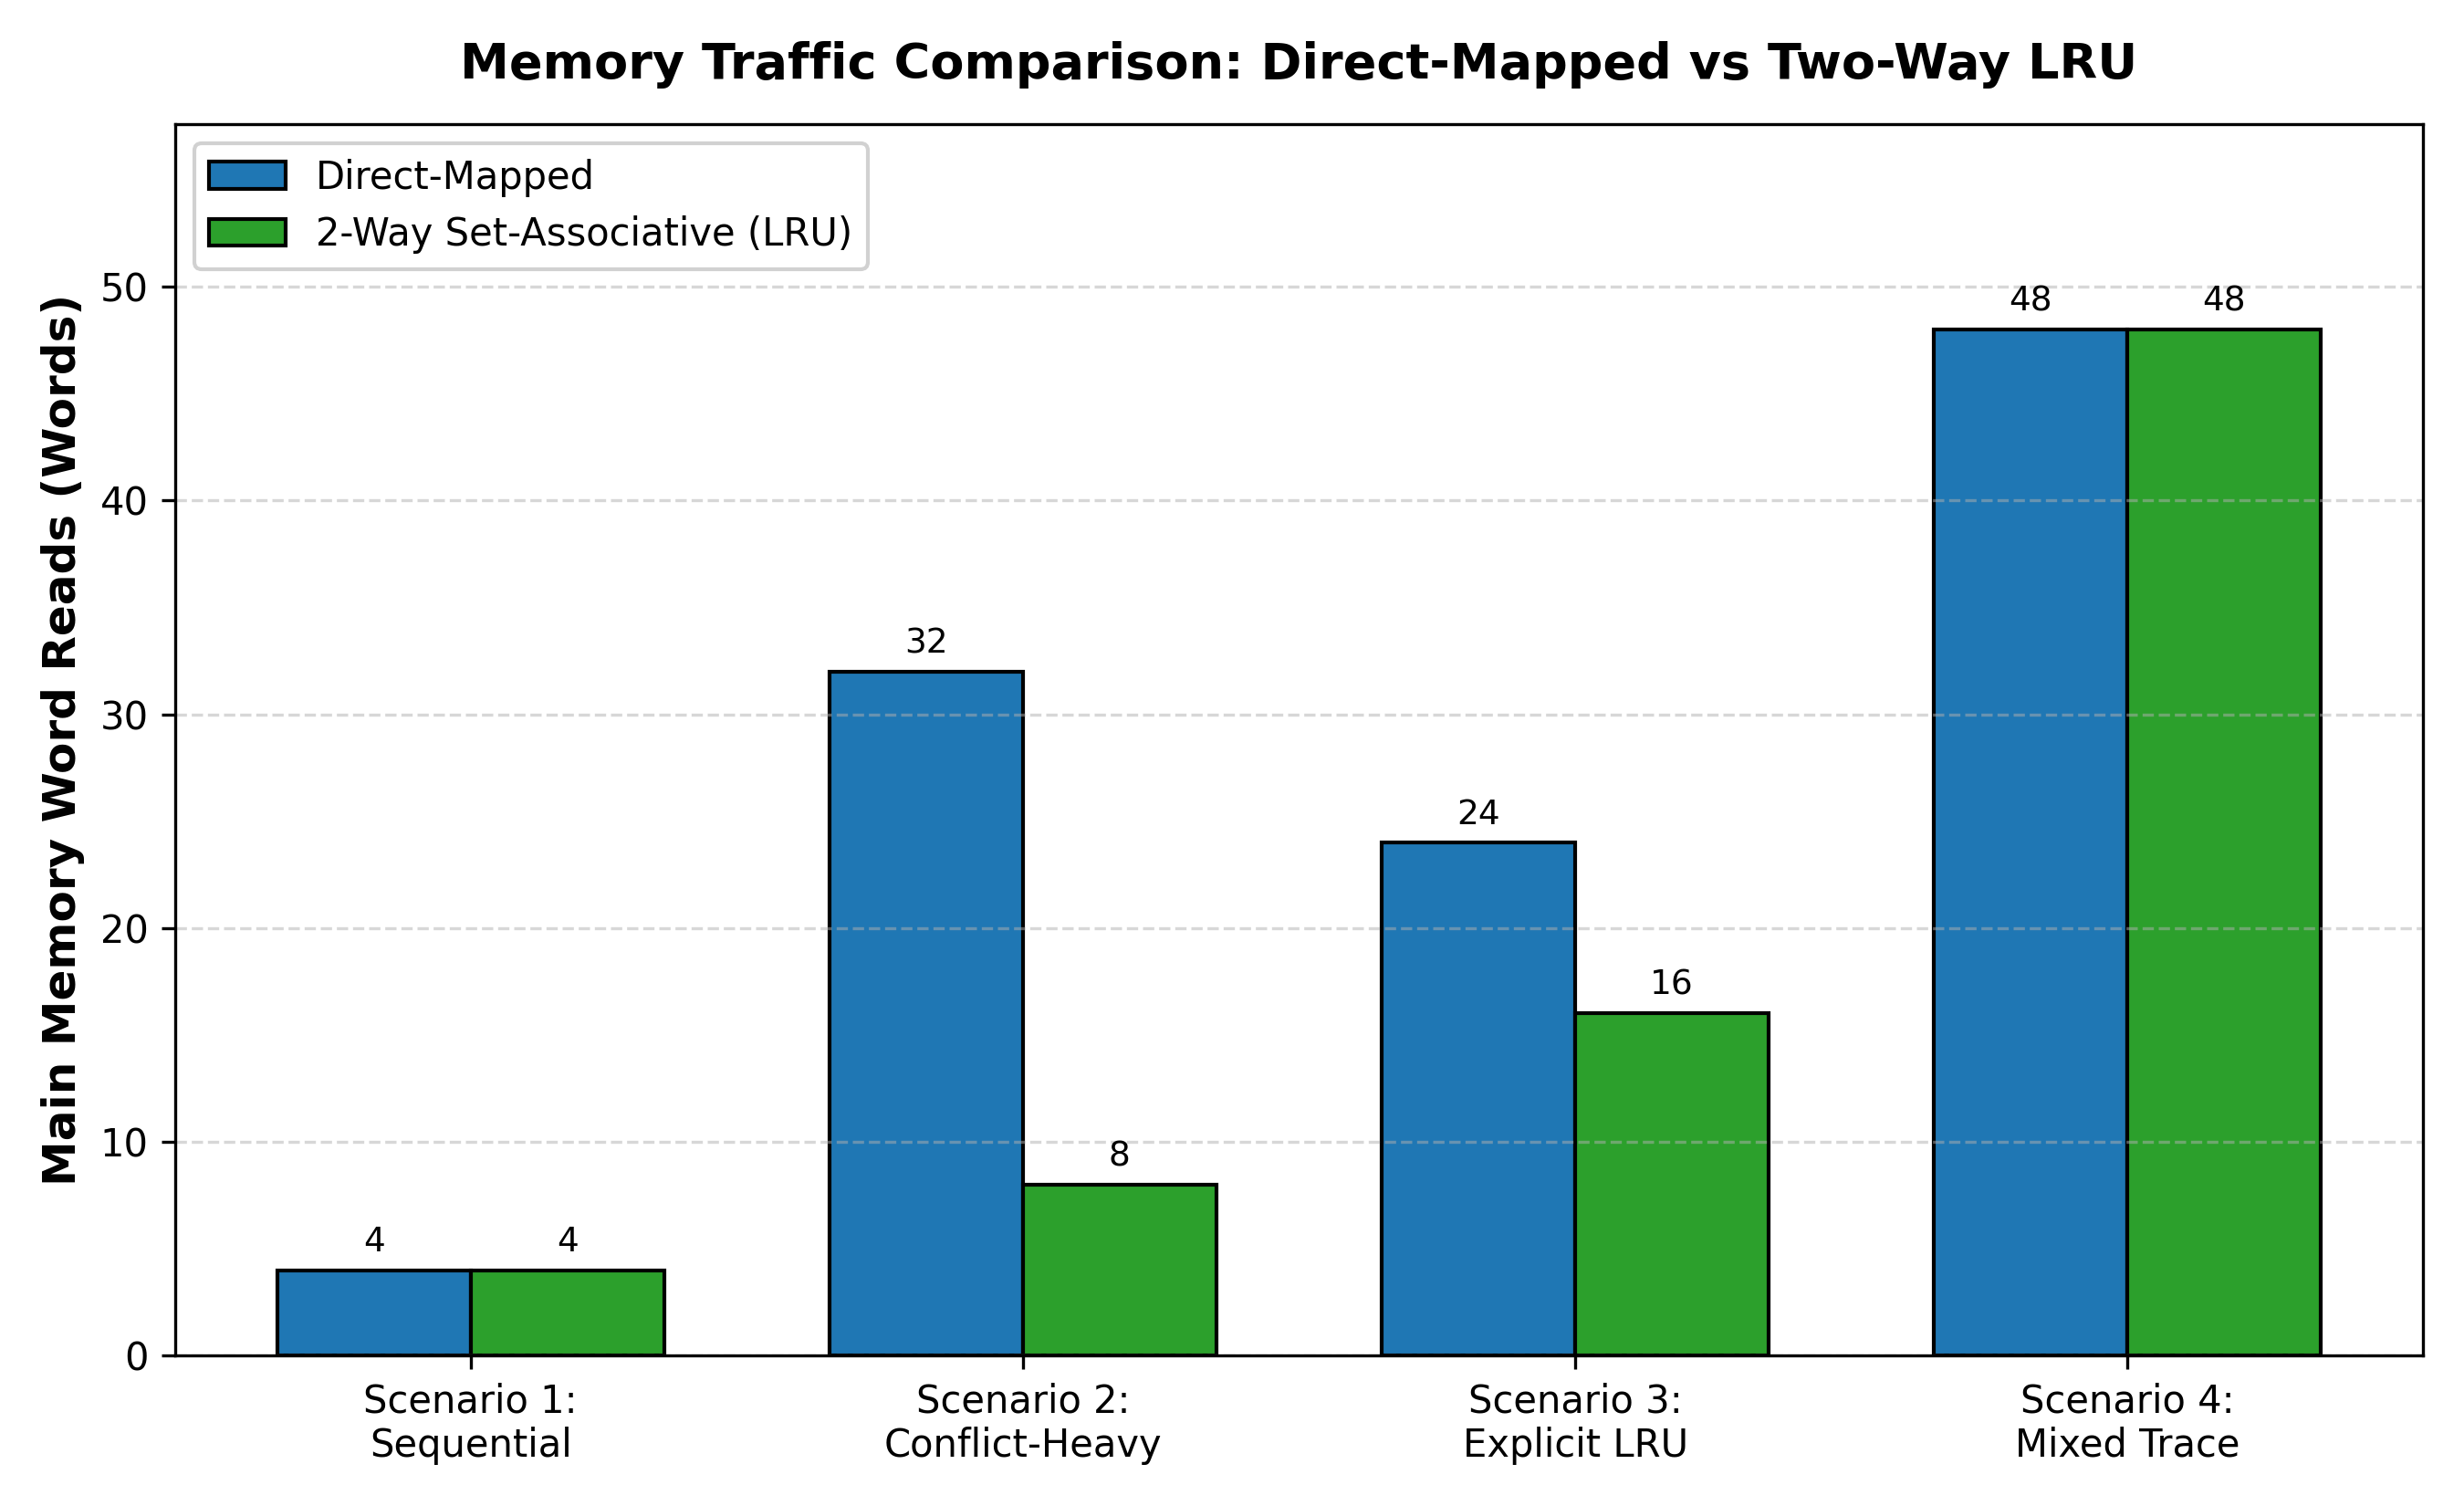
\includegraphics[width=0.92\linewidth]{memory_reads_comparison.png}
  \vspace{0.15em}
  \centerline{\small (c) Simulated Main-Memory Word Reads}
\end{minipage}
\caption{Empirical comparative performance metrics across all four synthetic benchmark scenarios: (a) hit rate (\%), (b) average access latency (cycles per completed access), and (c) simulated main-memory word read operations, highlighting the 75\% memory read reduction and 64.29\% latency reduction ($2.80\times$ speedup) under conflict thrashing.}
\label{fig:perf_comparisons}
\end{figure*}

\begin{table*}[t!]
\caption{Complete Measured Experimental Results Across All Benchmark Scenarios}
\label{tab:experimental_results}
\centering
\resizebox{\textwidth}{!}{%
\begin{tabular}{llcccccccc}
\toprule
\textbf{Scenario Description} & \textbf{Cache Architecture} & \textbf{Accesses} & \textbf{Hits} & \textbf{Misses} & \textbf{Hit Rate} & \textbf{Miss Rate} & \textbf{Sim. Mem Reads} & \textbf{Cycles} & \textbf{Avg Latency} \\
\midrule
\textbf{Scenario 1: Sequential} & Direct-Mapped & 4 & 3 & 1 & 75.00\% & 25.00\% & 4 & 27 & 6.75 cyc/acc \\
(Spatial Locality) & Two-Way Set-Assoc. & 4 & 3 & 1 & 75.00\% & 25.00\% & 4 & 27 & 6.75 cyc/acc \\
\midrule
\textbf{Scenario 2: Conflict-Heavy} & Direct-Mapped & 8 & 0 & 8 & 0.00\% & 100.00\% & 32 & 140 & 17.50 cyc/acc \\
(Thrashing Pattern) & Two-Way Set-Assoc. & 8 & 6 & 2 & \textbf{75.00\%} & \textbf{25.00\%} & \textbf{8} & \textbf{50} & \textbf{6.25 cyc/acc} \\
\midrule
\textbf{Scenario 3: Explicit LRU} & Direct-Mapped & 6 & 0 & 6 & 0.00\% & 100.00\% & 24 & 102 & 17.00 cyc/acc \\
(3-Address Trace: $ABACAB$) & Two-Way Set-Assoc. & 6 & 2 & 4 & \textbf{33.33\%} & \textbf{66.67\%} & \textbf{16} & \textbf{72} & \textbf{12.00 cyc/acc} \\
\midrule
\textbf{Scenario 4: Mixed Trace} & Direct-Mapped & 16 & 4 & 12 & 25.00\% & 75.00\% & 48 & 216 & 13.50 cyc/acc \\
(Realistic Access Sequence) & Two-Way Set-Assoc. & 16 & 4 & 12 & 25.00\% & 75.00\% & 48 & 216 & 13.50 cyc/acc \\
\bottomrule
\end{tabular}%
}
\end{table*}

\subsection{Experimental Setup and Verification Methodology}
The verification suite is executed using Icarus Verilog (v12.0) with standard IEEE 1800-2012 flags (\texttt{-g2012 -Wall}). Both the direct-mapped cache and the 2-way set-associative cache are instantiated in parallel inside \texttt{tb/tb\_cache\_comparison.sv} and driven concurrently by identical access traces.

The testbench incorporates two key verification features:
\begin{enumerate}
    \item \textbf{Address Poisoning}: After a request is accepted on \texttt{cpu\_req\_ready}, the address bus is overwritten with \texttt{32'hFFFF\_FFFF} on the subsequent negative clock edge. This confirms that the cache registers latch the address correctly and do not suffer from transparent latch leakage.
    \item \textbf{Response Backpressure}: The testbench artificially delays asserting \texttt{cpu\_resp\_ready} for multiple clock cycles, verifying that the cache holds \texttt{cpu\_resp\_valid} and \texttt{cpu\_resp\_data} stable without dropping transactions.
\end{enumerate}

Every completed access validates two hardware invariants:
\begin{align}
\text{hit\_count} + \text{miss\_count} &= \text{Total Completed Accesses} \\
\text{mem\_word\_read\_count} &= 4 \times \text{miss\_count}
\end{align}
Failure of either invariant triggers an immediate simulation \texttt{\$fatal} termination.

\subsection{Quantitative Benchmark Results}
We evaluate both caches across four synthetic access traces:
\begin{itemize}
    \item \textbf{Scenario 1: Sequential Spatial Locality (4 Accesses)}: Sequential word reads within the identical 16-byte block: addresses \texttt{0x00000000}, \texttt{0x00000004}, \texttt{0x00000008}, and \texttt{0x0000000C}.
    \item \textbf{Scenario 2: Conflict-Heavy Trace (8 Accesses)}: Alternating references between two addresses that map to the identical cache set: \texttt{0x00000000} and \texttt{0x00000080} repeated four times.
    \item \textbf{Scenario 3: Explicit Three-Address LRU Validation (6 Accesses)}: A canonical sequence $A \to B \to A \to C \to A \to B$ where $A = \texttt{0x00000000}$, $B = \texttt{0x00000080}$, and $C = \texttt{0x00000100}$. All three blocks map to Set~0 in the 2-way cache and Line~0 in the direct-mapped cache.
    \item \textbf{Scenario 4: Mixed Workload Trace (16 Accesses)}: A multi-set trace exercising spatial locality and temporal reuse across Sets 0, 1, and 2.
\end{itemize}

Table~\ref{tab:experimental_results} presents the measured simulation results exported to \texttt{results/results.csv}.

\subsection{Architectural Discussion}

\subsubsection{Scenario 1: Sequential Spatial Locality}
In Scenario~1, both architectures exhibit identical performance: 3 hits and 1 miss (75.00\% hit rate), requiring 4 simulated memory word reads and 27 clock cycles (6.75 cycles/access). The initial access to address \texttt{0x00000000} causes a compulsory cold miss. The cache controller fetches four consecutive 32-bit words, populating the entire 16-byte line. Subsequent accesses to offsets \texttt{0x4}, \texttt{0x8}, and \texttt{0xC} hit in the cache, requiring single-cycle lookups. This demonstrates the spatial locality benefit of multi-word lines, amortizing miss penalties over subsequent words.

\subsubsection{Scenario 2: Conflict-Heavy Thrashing Elimination}
Scenario~2 illustrates the impact of set associativity when resolving two-address conflict thrashing. Addresses \texttt{0x00000000} and \texttt{0x00000080} both have index bits \texttt{3'b000} in the direct-mapped cache, but differing tags (\texttt{0x000000} versus \texttt{0x000001}). In the direct-mapped cache, every single access evicts the resident block loaded by the immediately preceding access. This thrashing results in 8 misses out of 8 accesses (0.00\% hit rate), triggering 32 simulated memory word reads and consuming 140 clock cycles (17.50 cycles/access).

In the 2-way set-associative cache, both addresses map to Set~0 (\texttt{set\_idx = 2'b00}), with tags \texttt{0x000000} and \texttt{0x000002}. During the first two accesses, address \texttt{0x00000000} populates Way~0 and address \texttt{0x00000080} populates Way~1 via the invalid-first allocation rule. For the remaining six accesses, both lines reside simultaneously in Set~0. Consequently, accesses 3 through 8 result in cache hits. The 2-way cache achieves:
\begin{itemize}
    \item Hit rate increase from 0.00\% to 75.00\%.
    \item Simulated main-memory word reads reduced from 32 to 8 (a \textbf{75.00\% reduction} in simulated memory bus traffic).
    \item Measured execution latency reduced from 140 cycles to 50 cycles (a \textbf{64.29\% latency reduction}, corresponding to a $\mathbf{2.80\times}$ speedup ratio: $140 / 50 = 2.80$).
\end{itemize}

\subsubsection{Scenario 3: Deterministic LRU Eviction Proof}
Scenario~3 validates the exact cycle-by-cycle correctness of the 1-bit LRU controller. The step-by-step state trace is detailed in Table~\ref{tab:lru_trace}.

\begin{table}[htbp]
\caption{Cycle-by-Cycle Trace of Scenario 3 ($A \to B \to A \to C \to A \to B$)}
\label{tab:lru_trace}
\centering
\resizebox{\columnwidth}{!}{%
\begin{tabular}{ccccccc}
\toprule
\textbf{Step} & \textbf{Addr} & \textbf{Result} & \textbf{Set 0 Contents} & \textbf{LRU Bit} & \textbf{Victim} & \textbf{Outcome} \\
\midrule
1 & $A$ & Miss & Way 0: $A$, Way 1: Inv & 1 & Way 1 & Way 0 filled with $A$ \\
2 & $B$ & Miss & Way 0: $A$, Way 1: $B$ & 0 & Way 0 & Way 1 filled with $B$ \\
3 & $A$ & \textbf{Hit} & Way 0: $A$, Way 1: $B$ & \textbf{1} & \textbf{Way 1} & Way 0 hit; LRU set to 1 \\
4 & $C$ & Miss & Way 0: $A$, Way 1: $C$ & 0 & Way 0 & \textbf{$B$ evicted by $C$} \\
5 & $A$ & \textbf{Hit} & Way 0: $A$, Way 1: $C$ & 1 & Way 1 & Way 0 hit; $A$ preserved \\
6 & $B$ & Miss & Way 0: $A$, Way 1: $B$ & 0 & Way 0 & \textbf{$C$ evicted by $B$} \\
\bottomrule
\end{tabular}%
}
\end{table}

When block $C$ is accessed at Step~4, both ways in Set~0 are valid. Because block $A$ was hit in Step~3, the LRU bit points to Way~1 ($B$) as the victim. Thus, $C$ overwrites $B$, leaving $A$ intact in Way~0. At Step~5, the access to $A$ results in a confirmed cache hit, proving that LRU correctly preserved the most recently referenced block. At Step~6, accessing $B$ causes a miss because $B$ was previously evicted. Because Step~5 was an access to Way~0 ($A$), the LRU bit at Step~6 points to Way~1 ($C$) as the replacement candidate. Therefore, block $B$ is refilled into Way~1, evicting $C$. The expected final state of Set~0 is \textbf{Way 0 = $A$ and Way 1 = $B$, with $C$ evicted}. Across the six-access sequence ($A \to B \to A \to C \to A \to B$), the 2-way set-associative cache achieves a 33.33\% hit rate with confirmed hits at Steps 3 and 5, and misses at Steps 1, 2, 4, and 6. In contrast, the direct-mapped cache suffers a 100\% miss rate across all 6 accesses (0 hits, 6 misses, 24 simulated memory word reads, 102 cycles) because every reference evicts the preceding line.

\subsubsection{Scenario 4: Mixed Workload Dynamics}
Scenario~4 exercises a deterministic 16-access mixed workload: \texttt{0x00000200}, \texttt{0x00000204}, \texttt{0x00000210}, \texttt{0x00000220}, \texttt{0x00000280}, \texttt{0x00000300}, \texttt{0x00000200}, \texttt{0x00000380}, \texttt{0x00000210}, \texttt{0x00000400}, \texttt{0x00000224}, \texttt{0x00000500}, \texttt{0x00000300}, \texttt{0x00000580}, \texttt{0x00000200}, and \texttt{0x00000210}. Both caches exhibit identical macroscopic performance: 4 hits and 12 misses (25.00\% hit rate, 48 simulated memory word reads, 216 execution cycles).

Using one-based access numbering consistently across the trace, the four confirmed hits are:
\begin{itemize}
    \item \textbf{Access 2 (\texttt{0x00000204})}: Cache hit in Set~0 due to spatial locality within the 16-byte block refilled at Access~1.
    \item \textbf{Access 9 (\texttt{0x00000210})}: Cache hit in Set~1 due to temporal reuse of the line loaded at Access~3.
    \item \textbf{Access 11 (\texttt{0x00000224})}: Cache hit in Set~2 due to spatial locality within the block loaded at Access~4.
    \item \textbf{Access 16 (\texttt{0x00000210})}: Cache hit in Set~1 due to secondary temporal reuse of the line preserved in Set~1.
\end{itemize}

A detailed architectural analysis clarifies the nature of the 12 misses:
\begin{enumerate}
    \item \textbf{Compulsory (Cold) Misses}: The 16 accesses reference nine distinct 16-byte memory blocks. Across their initial references (Accesses 1, 3, 4, 5, 6, 8, 10, 12, and 14), both caches experience unavoidable compulsory misses to bring previously unreferenced blocks into storage.
    \item \textbf{Per-Set Conflict Misses}: Eleven of the 16 accesses map specifically to Set~0, referencing seven distinct blocks (\texttt{0x200}, \texttt{0x280}, \texttt{0x300}, \texttt{0x380}, \texttt{0x400}, \texttt{0x500}, \texttt{0x580}). In the direct-mapped cache, every new block mapping to Set~0 evicts the sole resident line. In the 2-way set-associative cache, Set~0 provides only two ways; because the number of concurrently competing blocks in Set~0 exceeds two, repeated evictions occur within Set~0 (causing misses at Accesses 7, 13, and 15), despite Sets 1, 2, and 3 having vacant or underutilized capacity.
    \item \textbf{Working Set vs. Footprint Distinction}: While the cumulative footprint of the nine unique blocks accessed over the entire execution trace equals $9 \times 16 = 144$ bytes (which exceeds the 128-byte cache capacity), this represents a cumulative reference footprint rather than the simultaneously active working set at any single point in time. In an analytical reference model of an idealized 8-line fully associative cache with LRU replacement (a derived analytical benchmark, not an RTL measurement), replaying this exact 16-access trace yields 9 misses and 7 hits (confirmed hits at Accesses 2, 7, 9, 11, 13, 15, and 16). All 9 misses in the fully associative reference are strictly compulsory (cold) misses upon initial block touch, with 0 additional capacity misses. Consequently, comparing our measured RTL results (both direct-mapped and two-way set-associative caches exhibiting 4 hits and 12 misses) against the fully associative reference establishes that the two-way cache incurs exactly 3 additional conflict misses ($12 - 9 = 3$, at Accesses 7, 13, and 15) due to Set~0 contention, rather than capacity exhaustion.
\end{enumerate}

\subsection{Structural Hardware Comparison}
Table~\ref{tab:complexity_tradeoffs} provides a structural comparison of hardware resources based on the RTL implementation.

\begin{table}[htbp]
\caption{Microarchitectural Structural Resource Comparison}
\label{tab:complexity_tradeoffs}
\centering
\renewcommand{\arraystretch}{1.25}
\resizebox{\columnwidth}{!}{%
\begin{tabular}{lcc}
\toprule
\textbf{Hardware Resource} & \textbf{Direct-Mapped Baseline} & \textbf{2-Way Set-Associative} \\
\midrule
Tag Comparators & $1 \times 25$-bit & $2 \times 26$-bit (Parallel) \\
Tag Storage Overhead & $8 \times 25 = 200$ bits & $8 \times 26 = 208$ bits \\
Valid Bits & 8 bits (1 per line) & 8 bits (1 per way) \\
Replacement Storage & 0 bits & 4 flip-flops (1 bit/set) \\
Data Multiplexing Logic & 4-to-1 Word MUX & 2-Way Hit MUX + 4-to-1 MUX \\
Addressing Organization & 8 lines (3-bit line index) & 4 sets (2-bit set index) \\
Critical Path Delay Components & Single Tag Match & Parallel Tag Match + Way MUX \\
\bottomrule
\end{tabular}%
}
\end{table}

\textit{Implementation and Simulation Note}: In this investigation, cycle-accurate RTL simulation was performed using Icarus Verilog to verify functional correctness and timing behavior. FPGA logic synthesis, placement, routing, and physical board programming were not performed. The comparisons in Table~\ref{tab:complexity_tradeoffs} represent structural RTL design properties. Neither commercial FPGA synthesis toolchains nor open-source synthesis tools were executed. All SystemVerilog modules have been authored strictly adhering to standard synthesizable RTL design principles (synchronous edge-triggered registers, separate blocking assignments for combinational logic, non-blocking assignments for state registers, and explicit default cases to prevent unintended transparent latches), ensuring clean synthesizability for future physical hardware evaluation.

% -----------------------------------------------------------------------------
% Section VI: Team Roles and Contributions
% -----------------------------------------------------------------------------
\section{Team Member Roles and Engineering Contributions}
\label{sec:contributions}

The project research team comprises five student investigators at the Department of Computer Science and Artificial Intelligence, Newton School of Technology: Satyam Kumar, Krishna Verma, Akshit Vats, Chinmay Soni, and Lakshya Bapna. The core hardware implementation was structured into four primary modular work packages, alongside cross-functional verification, benchmark data analysis, and technical documentation. Based on repository commit records and engineering deliverables, the technical roles are structured as follows:

\begin{itemize}
    \item \textbf{Satyam Kumar} (Member 3): Designed and implemented the standalone 1-bit LRU replacement controller (\texttt{rtl/lru\_controller.sv}) with invalid-first allocation priority. Architected the 5-state blocking cache FSM controller (\texttt{cache\_2way\_controller.sv}) managing handshakes, burst refills, and counter updates. Integrated the structural top-level wrapper (\texttt{cache\_2way\_top.sv}) and authored unit and smoke verification testbenches (\texttt{tb/tb\_lru\_controller.sv}, \texttt{tb/tb\_cache\_2way\_smoke.sv}).
    \item \textbf{Krishna Verma} (Member 4): Developed the multi-cycle synchronous main memory simulation model (\texttt{sim/simple\_main\_memory.sv}) with parameterized access latency. Authored the unified comparative benchmarking testbench (\texttt{tb/tb\_cache\_comparison.sv}) driving concurrent traces. Developed the automated data analytics pipeline (\texttt{analysis/analyze\_results.py}) and generated comparative performance plots.
    \item \textbf{Akshit Vats} (Member 5): Conducted benchmark invariant verification across all access traces, verifying mathematical hardware invariants ($\text{hits} + \text{misses} == \text{accesses}$ and $\text{sim\_mem\_reads} == 4 \times \text{misses}$). Coordinated empirical results auditing and academic documentation deliverables.
    \item \textbf{Chinmay Soni} (Member 1): Developed the foundational SystemVerilog package (\texttt{cache\_pkg.sv}) defining global architectural constants, address slices, and array dimensions. Implemented the complete 128-byte direct-mapped baseline cache (\texttt{direct\_mapped\_cache.sv}) featuring integrated valid/tag arrays, comparator, 4-word refill logic, and performance counters. Authored \texttt{tb/tb\_direct\_mapped.sv}.
    \item \textbf{Lakshya Bapna} (Member 2): Engineered the modular dual-way storage datapath (\texttt{cache\_2way\_datapath.sv}) containing Way~0 and Way~1 valid, tag, and data arrays across four sets. Implemented parallel 26-bit tag matching circuitry, hit detection logic, way multiplexers, and 4-to-1 word extraction multiplexers. Authored unit testbench \texttt{tb/tb\_cache\_2way\_datapath.sv}.
\end{itemize}



% -----------------------------------------------------------------------------
% Section VII: Conclusion and Future Work
% -----------------------------------------------------------------------------
\section{Conclusion and Future Work}
\label{sec:conclusion}

In this project, we designed, modeled, integrated, and empirically evaluated a 128-byte, 2-way set-associative cache with 1-bit LRU replacement against an identically configured direct-mapped baseline cache in IEEE 1800-2012 SystemVerilog. Experimental simulation confirms that two-way set associativity eliminates ping-pong cache thrashing under two-address conflict access patterns, elevating the hit rate from 0.00\% to 75.00\%, decreasing simulated main-memory word reads by 75.00\%, and reducing measured execution latency by 64.29\% (a $2.80\times$ speedup ratio). Furthermore, cycle-by-cycle testing of an explicit three-address conflict trace ($A \to B \to A \to C \to A \to B$) verified the deterministic correctness of our invalid-first allocation priority and 1-bit LRU tracking algorithm, establishing that the expected final set state is \textbf{Way 0 = $A$ and Way 1 = $B$, with $C$ evicted}.

\subsection{Future Work}
Building upon the verified read-only baseline established in this work, potential future architectural extensions include:
\begin{enumerate}
    \item \textbf{Write Policy Integration}: Implementation of write-through with write buffers and write-back with dirty bits (\texttt{dirty\_array}), requiring cache-line write-back FSM sequences to main memory.
    \item \textbf{Non-Blocking Cache Extensions}: Integration of Miss Status Holding Registers (MSHRs) to support hit-under-miss and miss-under-miss concurrency, enabling pipelined memory requests.
    \item \textbf{Higher-Order Associativity}: Exploration of 4-way set-associative configurations using Pseudo-LRU (tree-PLRU) replacement policies to assess area-latency scaling.
    \item \textbf{Physical Hardware Implementation}: Synthesis, placement, routing, and timing closure on an FPGA development board (e.g., AMD/Xilinx Artix-7) to measure exact Look-Up Table (LUT), Flip-Flop (FF), Block RAM (BRAM), and maximum operating frequency ($F_{\max}$) trade-offs under physical silicon constraints.
\end{enumerate}

% -----------------------------------------------------------------------------
% References
% -----------------------------------------------------------------------------
\bibliographystyle{IEEEtran}
\bibliography{references_phase2}

\end{document}
